\section{Results}

\subsection{Editors/Articles Ranking Calibration}

\subsection{Interpretation of the Biased Random Walker Calibration for each Category}


\subsection{Correlations with exogenous variables}

To understand the results, we must have a firm grasp on what $\alpha$ and $\beta$ mean. They are more easily understood by roughly rewriting $\mathbf{w^*}$ as:
\begin{equation}
\begin{cases}
w^{*}_{e} \sim k^{1-\beta}_{e} \langle k_{a}^{-\alpha}\rangle_e \\

w^{*}_{a} \sim k^{1-\alpha}_{a} \langle k_{e}^{-\beta}\rangle_a
\end{cases} \label{eqsim}
\end{equation}

Here we can see the similarity of $w^*$ is related to the product of two expression. Values of $\alpha$ and $\beta$ can make the one of the product close to one or and so the other parameter may dominate.

The results of calibrating our model are encouraging as we find high correlations between the results of our $w^*_e$ algorithm and our exogenous variables $v$. 

We define $\rho$ at the maximum achievable spearman rank correlation between $w^*$ and $v$ for editors or articles, by category, and over time. The variation of $\rho$, by for editor for any category ranges from 0.75 to 0.46 with a mean 0.64.  That same statistic for articles is articles from 0.91 to 0.57 with a mean of 0.72, which is overall higher.

 
From snapshotting we see view $\rho$ as  a function of time. In the case of editors we see increasing trends in all categories over time. This means that $w^*_e$ benefits from incorporating more contribution history. As for articles, from the start of a category's history the correlations remain stable. \ref{fig:rhotime}

\begin{figure}[!t]
\centering
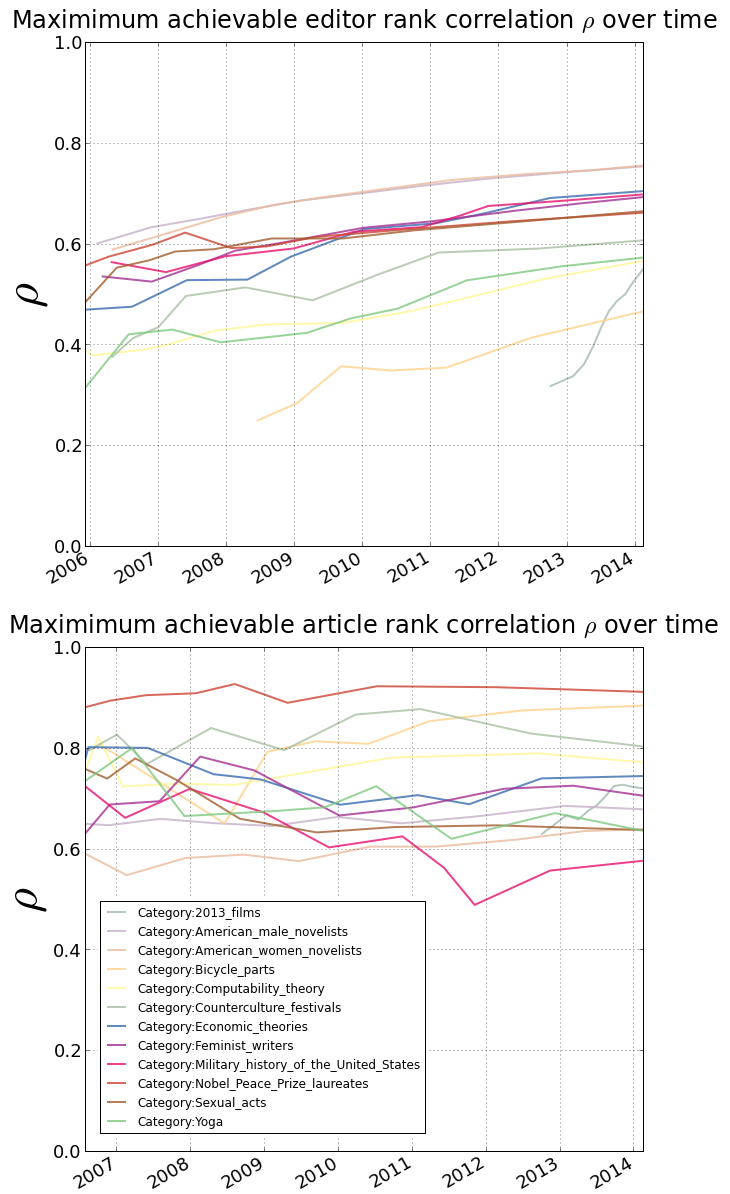
\includegraphics[width=0.9\columnwidth]{Figures/rho_combined.png}.
\caption{$\rho$ over time, by category and type}
\label{fig:rhotime}
\end{figure}


%$\alpha$ is a measure of how important it is for quality that many users edit, with lower alpha, we have a more collaborative category, where edits are more equal and egalitarean. With alpha high, the category is more rewarding users that operate more individualistically. Beta is inversely related to alpha so the same can be said but the directions of the arguments reversed. This means we can talk of the characteristic of a category, compared to one another and compared over time. 

\subsection{Negative values of $\alpha$ and $\beta$}
Another surprising result is that we find at times, negative values for $\alpha$ and $\beta$.


For editors, maximum $\rho$ always occurs strictly within a radius of 0.01 around the origin on the  $\alpha$-$\beta$ plane. The $(0,0)$ solution is significant in that it represents unbiased arithmetic averages.
\ref{fig:landscape}

For articles, the solutions have 2-dimensional unbounded triangular solution space. For instance in Category:Economic Theories we find a typical solution space\ref{fig:landscape} . This solution space indicates that the behaviour displayed by the  landscape is a spectrum of possibilities. One one extreme that either $\alpha$ is positive but small, in which case $\beta$ is bounded tightly, which means that fitter editors are producing more obscure articles. Or that $\alpha$ is negative and that $\beta$ is less bounded. This indicates that $\alpha$ is dominating, as is the case in \eqref{eqsim}, and that less fit editors are contributing more, and the ubiquity of their contributions is relatively unimportant. Between categories variations in triangular solution space are rotations around the origin. In our particular example we also find that this solution space is rotated towards the positive $\beta$ axis. So even as the trade triangle occurs, its favours positive $\beta$. Interpreted means that editors who edit relatively more obscure articles are important to success of articles in Category Economic Theories. We do not encounter any rotation in any category that would be large enough to be equivalent to a reflection across the $\alpha = \pm \beta$ axes.

\begin{figure}[!t]
\centering
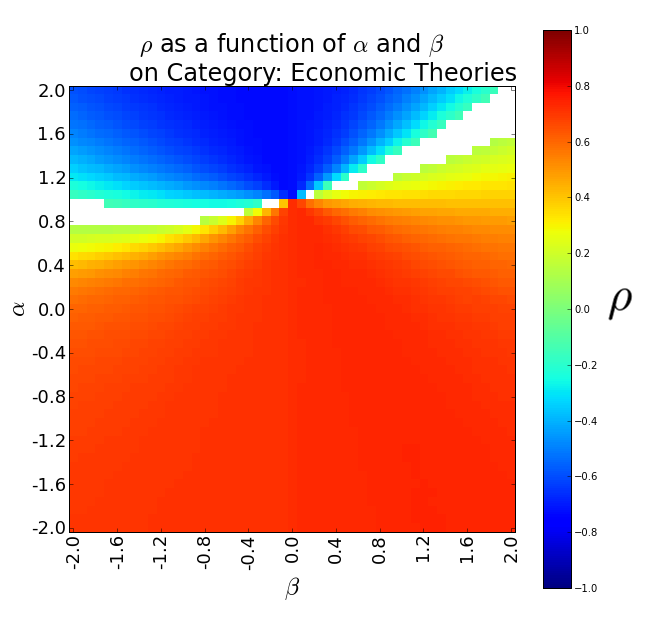
\includegraphics[width=0.9\columnwidth]{Figures/landscape.png}.
\caption{Landscape}
\label{fig:landscape}
\end{figure}

